% !TEX root = ../thesis-example.tex
%
%personal perception and interaction with medical information
\chapter{Introduction}  %6 pages
\label{sec:introduction}
Medicine is the science and practice of the diagnosis, treatment, and prevention of disease, and most medical information is about our human body. Kinds of medical information are employed in different procedures, such as education, training, diagnosis, operation, and so on. 
As the computing technologies develop, more and more information is digitized from the physical world, and then researchers work on how to process and show them back to the user, enabling the user to perceive and interact with the information naturally and effectively. 
Perception and interaction with different media and objects are the fundamental human activities, and they are, meanwhile, user specific \cite{Turk2000}.
In this thesis, we do research on the personalized perception and interaction with the medical information during education, operation and so on. 
Mixed Reality (MR) tries to blur the boundary between the real world and the virtual world, generated based on the digital information, to improve the perception and interaction experience \cite{Kruijff2010}.
Human centered computing aims at adapting computers to human minds and habits, and an important research direction in this area is the design of user interface. 
A perfect user interface should automatically adjust to the engaged user's personality. 
A MR framework for personalized perception of medical information is proposed for medical education and rehabilitation exercise, and pointing gestures are employed for the user interacting with ambient media and objects in an egocentric setting. Finally, these two techniques are combined to create a framework for collaborative MR.
%limited by real world, Virtual reality, AR and MR to improve the perception and simple learning procedure
%sterile rule and physical fact, nornal interaction => natrual interaction with pointing and hand gestrue  

\section{Motivation}
The foundation for the motivation of this work is the recent developments in Mixed Reality. Different MR applications are developed for medical education, training, and intra-operative navigation, and these techniques enable more intuitive perception of the medical information and instinctive interaction with different medical information. 
In the following paragraphs a short overview of the current challenges and motivations for each topic are presented. 

\subsection{Personalized perception of medical information}
\paragraph{Challenges for anatomy education}
Anatomical education is an important content of every curriculum and starts already very early in school, to form a good understanding of the body and improve the general health awareness \cite{Dunnill2013}. In today's medical schools, students are required to understand both function and spatial context of human anatomy. Traditional medical education learning is classified into three categories: cadaver, model, and book-based. The cadaver-based learning has seen decline due to practical and cost issues. As a result, anatomical education has shifted towards diagram, physical, and virtual models. However, some drawbacks exist with these learning paradigms. For example, it is difficult to interpret the spatial and physical characteristics of anatomy by observing two-dimensional images, diagrams, or photographs. Many physical models also lack detail levels to fully understand the specific anatomy. 
Numerous digital anatomy models exist and these resources are very valuable. The disadvantage is that the user still has to mentally map/link anatomy onto the human bodies.
Providing adequate learning experience to different learners is also a challenging issue as the traditional learning system generally does not adapt content to suit individual learner needs.
With the advent of the plethora of exciting technological advancements there should be no reason not to include these for the creation of new education paradigms for medical learning. 

\paragraph{Challenge for motor rehabilitation}
Motor rehabilitation restores a patient's functional health that is damaged due to musculoskeletal or nervous system impairments. It consists in iterative repeating exercises to strengthen the affected body area. It requires movements to be performed in a very specific way, otherwise the gain may not be adequate and the desired results will be less noticeable \cite{Merians2006,Ustinova2014}. Often, since the rehabilitation must be performed over quite a long period it is common for patients to get disinterested, and consequently, they perform the exercises in a casual and incorrect manner. Usually, Motor rehabilitation occurs by regular meetings between patient and physiotherapist with frequency depending on the availability of both. The time that patients spend on therapy in clinics is very short compared to the potential time that they can spend on it outside of the clinical setting (\eg at home). Thus, we believe that it becomes crucial for the patient to perform exercises at home to speed up the rehabilitation process. However, both therapeutic instructions and corrections by the therapist are not verbally provided to the patient at home and it potentially leads the patient to perform the exercises incorrectly.

\paragraph{Mixed Reality for education and serious gaming}
MR systems have the advantage that digital information can be embedded and/or superimposed upon reality. This allows for a more close-to-reality presentation of medical knowledge and offers opportunities for new and interactive learning context. 
The user can spatially relate corresponding medical information to the reality objects, \eg human body. 
The main reason for MR not being used in many systems today is that developing MR systems is more challenging than developing virtual reality systems. 
The integration of real and virtual objects requires accurate calibration, more advanced visualization and special user interfaces.
Personalization for promoting a multi-modal learning environment is also a growing area of interest, such as the development of user modeling and personalized processes which place the user at the center of the learning environment.
The concept of ``Magic Mirror'' is that the user stands in front of a screen and via a camera, the image of the user is shown on the screen such that it acts like a mirror. While such a system restricts the motion of the user, it allows for an inexpensive and robust solution that is better suited for medical education and serious gaming.  

\subsection{Natural interaction in operating room}
\paragraph{Challenges for interaction in operating room}
As medical technology is continuously developing, more medical systems are integrated inside the operating room (OR) for diagnosis and intra-operative navigation. Today, the conventional display technology in the operating room is still the 2D display and the information from different medical systems is shown on different displays.
\figurename{\ref{fig:1-intro:ORScenario}} showcases the photo of a modern day operating room at Klinikum der Universit\"at M\"unchen - Campus Gro{\ss}hadern that consists of six unique displays for different medical information output. 
Surgeons rely on these medical systems to capture, browse, and manipulate patient information, physiological data, and medical images, but the current control input of these systems are still mouse, keyboard, touch screen, and joystick. To interact with these medical systems and their control inputs, the user has to press either a physical/virtual button using their own finger or a visual cursor controlled by another device. 
Yet, one of the most important rules in the OR is to maintain a strict boundary between what is sterile and what is not \cite{OHara2014a}. A sterile processing of the input devices is impossible; hence the surgeons cannot directly touch these input devices after they are scrubbed and gloved. However, research shows that the surgeon {needs} to directly control the medical systems to mentally `get to grips' to what is going on, something which is not achievable by proxy \cite{Johnson2011a}. In addition, the input devices of different systems are totally independent due to security and privacy rules. The management of multiple interfaces in the modern operating room is also a challenge for the nurse and surgeon.
\begin{figure} [htb]
	\centering
	% Use the relevant command to insert your figure file.
	% For example, with the graphicx package use
	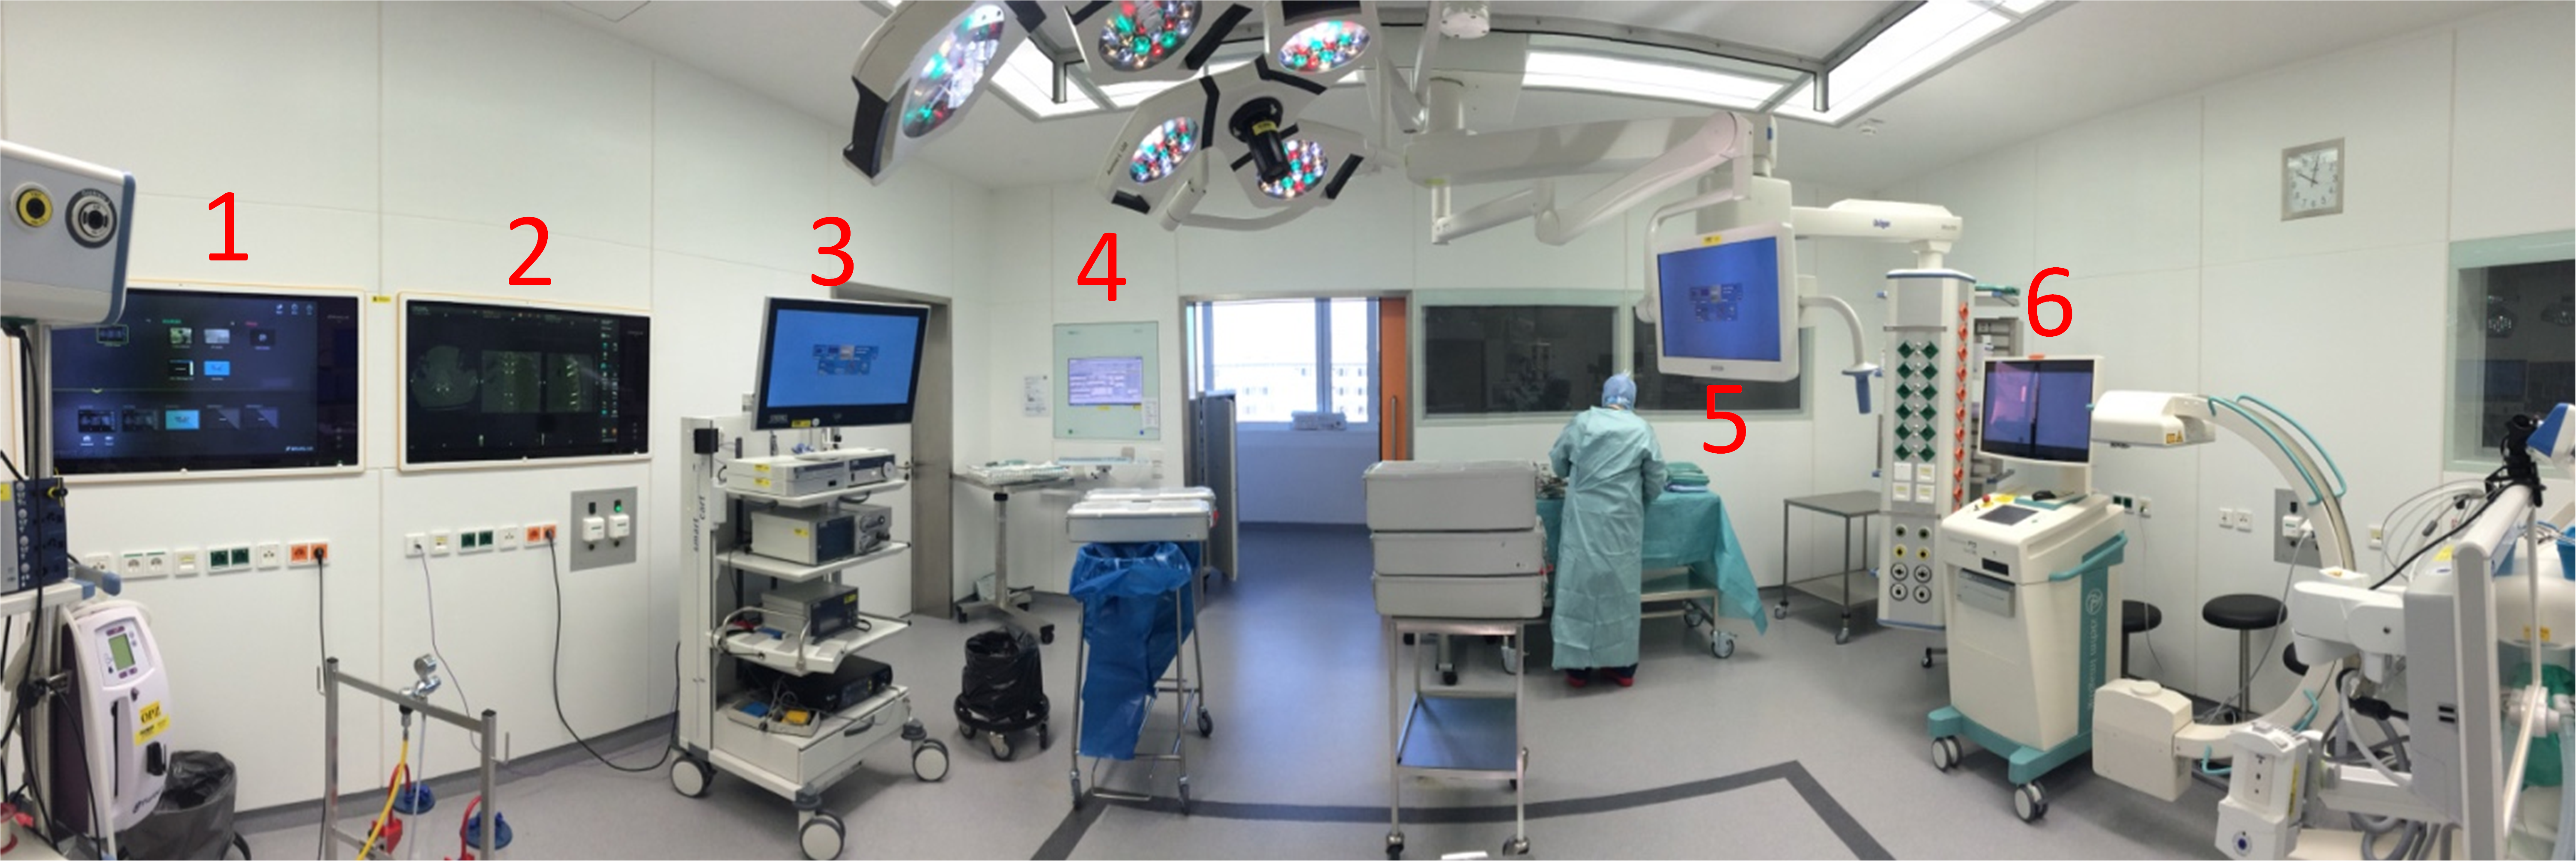
\includegraphics[width=1.0\textwidth]{figures/4-PointingOR/ORScenario}
	% figure caption is below the figure
	\caption{There are six displays in a normal operating room in Klinikum der Universit\"at M\"unchen - Campus Gro{\ss}hadern for different medical systems. The function of these displays are 1\&2: DICOM images from the archive or live video streaming from the handle grip camera; 3: Arthroscopy Monitor; 4: SAP Hospital Information System; 5: Ample monitor sharing the same screen as 1 or 2; 6: Fluoroscopy monitor.}
	\label{fig:1-intro:ORScenario}       % Give a unique label
\end{figure}
\paragraph{Pointing gesture for interaction}
Human centered computing aims at adapting computers to human minds and habits, and an important research direction in this area is the design of natural and ergonomic human-computer interaction techniques.
Pointing gestures are fundamental to human behavior \cite{Matthews2012} and are used consistently across cultures  \cite{McNeill2000}. The gestures begin at an early developmental stage \cite{Carpendale2010} and let humans reference proximal objects as well as abstract concepts in the world. Today, pointing gestures are not only part of our gestural language but are inherently used for interaction \cite{Nanayakkara2013a}.
A few authors have tried to estimate the user's eye position and recover the \textit{eye-rooted} pointing geometry to enable interacting with ambient media and objects in the real world. One existing technique consists in positioning a camera next to the monitor or on the ceiling to observe the user and implement the outside-in tracking. In this case, the computing device calculates the eye position by detecting the user's gaze and face or wearable trackers. Unfortunately, the user has to stand within a limited working zone defined by the camera, as shown in \figurename{\ref{fig:1-intro:problem}(a)}.
As an alternative to the traditional setting of external sensors observing the user, the egocentric setting mounts a portable camera on the head or clothing of the user and perceives the interaction from an egocentric perspective \cite{Fathi2011,Li2015}. 
Other researchers have taken advantage of an egocentric setting employing inside-out tracking \cite{Harrison2011,Mistry2009}. 
% and enabling the user to perform pointing interaction with digital information .
They directly take the camera center as the pointing ray origin, as shown in \figurename{\ref{fig:1-intro:problem}(b)}. These methods work well when the user performs interaction with objects and media which are reachable.
However, what if the user tries to point towards objects which are not reachable (see \figurename{\ref{fig:1-intro:problem}(c)} ). There is a significant angle between the ray starting from the camera and that from the eye. Hence, there is an important offset between $O_{eye}$, the object which is pointed at in the user's view, and $O_{camera}$, the object observed in the camera view.
%As such, to calculate the eye position in an egocentric setting, cameras have to be mounted to track the eye gaze. Current solutions provide the user a real-time visual feedback.
\begin{figure} [htb]
	\centering
	\includegraphics[width= \linewidth]{figures/4-PAST/problem}
	\caption{The \textit{eye-rooted} pointing geometry in different setups. (a) There is a limited working zone when positioning a camera to observe the user. (b) The camera position can be chosen as the origin point when the desired object is reachable. (c) There is a significant angle between the ray starting from the camera and that from the eye when the target is unreachable.}
	\label{fig:1-intro:problem}
\end{figure}

\subsection{Collaborative characteristics}
Collaboration between people become more and more common when using computer. Human-Computer Interface (CHI) is giving away to a Human-Human Interface mediated by computers \cite{Billinghurst1999}. From the real world to a MR environment, there are functional seams and cognitive seams for the user during the cooperation. The normal interaction methods should be kept in the MR application, if possible.
There are new technical challenges to be addressed when there are more than one user in a common workplace.
%todo define the challenge and requirements
In normal anatomy teaching or rehabilitation scenario, there is a teacher or doctor to teach and monitor the student/patient for the learning and exercise. There are also several surgeons to control several medical systems during the operation. The challenge is to support the collaborative MR when we try to introduce the new techniques.
%In addition, the functions and user interface of a MR application is not so intuitive as mouse and keyboard. 

\section{Objectives}
The objectives of this work are to investigate the personalized Magic mirror framework, in order to improve the perception and interaction with digital medical information, and proposed pointing gesture recovery in an egocentric setting for natural interaction with ambient media and objects. At last there two technologies are integrated to create a framework for collaborative MR.
In the following listings the prime objectives are briefly highlighted.

\begin{description} [font=$\bullet$\scshape\bfseries]
	\item Develop a personalized MR magic mirror for medical education and motor rehabilitation, which improves the perception based on the personal information and natural interaction and motivates the user via gaming elements.%perform user studies to evaluate and find the suitable research directions.
	\item Propose a method to accurately recover the \textit{eye-rooted} pointing ray without tracking the eye gaze in an egocentric setting, enabling the user directly performing pointing gesture to interact with ambient media and objects without visual feedback.
	\item Introduce a novel user interface that allows the surgeon to personally perform touchless interaction with the various medical systems, and switch effortlessly among them, all of this without modifying the systems' software and hardware.
	\item Propose a collaborative MR framework for medical teaching and rehabilitation, which combines the personalized MR magic mirror and pointing gesture interaction in egocentric setting. 
\end{description}

\section{Contribution}
In the course of this thesis several solutions and methods have been contributed to personalized mixed reality and pointing gesture interaction, both for medical education, rehabilitation exercise and touchless operation with various medical systems.

\paragraph{Personalized perception in Magic Mirror framework}
A magic mirror framework is presented creating a MR environment with an \textit{in-situ} augmented reality (AR) view. The system can track the current user and finish the registration between the medical datasets and the user based on the personal information (e.g., height, body size, gender, and age). It inherently allows the user to perform interactive registration and directly map the medical information onto his/her body. This opens interesting possibilities for personalized mixed reality for medical education and rehabilitation exercise. Through the participation of 7 clinicians and 72 anatomy students, two user studies were designed to respectively assess the precision and acceptability of the magic mirror system for anatomy education in the classrooms of tomorrow. We also take the advantage of the interactive mixed reality to generate a personalized learning procedure. In addition, ``Organ Explosion'' and ``self-control virtual view'' systems are designed and implemented for anatomy leaning. Serious games are also developed in the framework for health-care education and rehabilitation exercise.

\paragraph{Pointing gesture recovery in an egocentric setting}  
A method is proposed to calculate a virtual eye center as the origin for the \textit{eye-rooted} pointing ray technique without tracking the eye gaze in an egocentric setting. The user specific pointing geometry can then be recovered for interaction with ambient media and objects without visual feedback. The pointing ray starts from the virtual eye center and goes through the fingertip to the desired target information. During the initial calibration, the user is asked to perform pointing gestures towards several targets displayed within the field of view. A user specific virtual eye center is then estimated based on the detected fingertip in the coordinate system of the wearable device. Then the \textit{eye-rooted} pointing ray is recovered when a user is performing a pointing gesture. 
%We provide both a mathematical validation and a user study involving ten participants to assess the precision of our unique pointing gesture recovery.
The proposed method is mathematically analyzed and determined that the calibration is feasible with a measured accuracy of the recovered pointing ray below $0.9\degree$.
The method is also evaluated in a user study consisting of 10 participants performing pointing interaction with objects shown on the display while wearing a RGB-D sensor. The study shows that the calibration is independent of the environment and the pointing ray is recovered with an accuracy of $0.67 \pm 0.71\degree$ without any visual feedback.

\paragraph{Natural interaction with multi-system in OR}
Contrary to the state-of-the-art, a novel user interface is introduced, allowing the surgeon to {personally} perform touchless interaction with the {various} medical systems, and switch effortlessly among them, all of this {without modifying} the systems' software and hardware. The advantages are: 

\begin{description} [font=$\bullet$\scshape\bfseries]
	\item needs no modification of the software/hardware of the existing medical systems and does not need the medical software to be re-certified
	\item combines pointing with personal gesture command
	\item switches smoothly among different medical systems and operands
	\item offers multi-user, multi-system framework
\end{description}

Android devices with a special application are connected to the computers on which the medical systems are running, simulating a normal USB mouse and keyboard. 
Based on the pointing gesture recovery technique, the surgeon's pointing gesture can be calculated. The target position in the real world, the desired cursor position in the display and the surgeon's personal gestures, are detected and analyzed. The result is sent to the Android devices via WiFi. The application running on the Android system generates the corresponding mouse or keyboard events according to the targeted medical system allowing completion of the interaction. In essence, one personal user interface is conceived to control all systems in an operating room.

\paragraph{Collaborative MR framework for teaching and rehabilitation}
A multi-user collaborative MR framework is introduced by integrating the MR magic mirror and the pointing gesture in egocentric setting.
The human-human communication is partly implemented via pointing gesture and MR framework. %, and the functional and cognitive seams are evaluated.
The framework is examined in two scenarios, anatomy teaching with a student and rehabilitation exercise with a nurse. The teacher directly points to the MR view and controls it to lead the teaching procedure, and the nurse in charge of the exercise in the same way.

\section{Organization}
In this thesis, issues related to improve the personalized perception and interaction are discussed and presented, and it is organized as the following. 
The state of art of perception and interaction with medical information, including medical education, rehabilitation, and intra-operative interaction and so on, is presented in Chapter \ref{sec:bg}. Furthermore, the history and the state of mixed reality and natural user interface using gestures is discussed.
In Chapter \ref{chaptor:3}, the magic mirror framework is presented and several methods are investigated to improve the user's perception in the magic mirror setting. Personal information is detected to select the best medical data for registration and personalized registration is performed to improve the AR view.  Several functions and applications are developed for medical education and rehabilitation.
In Chapter \ref{chapter:4}, a Point At Several Targets (PAST) method is proposed to calculate an origin for the \textit{eye-rooted} pointing gesture and recover the pointing ray in an egocentric setting. The proposed method is mathematically analyzed and evaluated in a 10 participants user study. A novel user interface for various medical systems in the operating room is presented based on the recovered pointing gesture. 
%The gesture method is extended to perform interaction in a normal scenario without any depth information. 
Then, a collaborated MR framework encompassing the magic mirror conception and the pointing gesture is proposed in Chapter \ref{chaptor:5}. 
%The framework is examined in the learning and rehabilitation scenarios. The teacher directly points to the MR view and controls it to leading the learning procedure, and the nurse in charge of the exercise at the same way.
%The scenario with multi-user performing magic mirror learning and rehabilitation and one nurse to monitor and supervise all the user at the same time and perform interaction with each MR application seamlessly with the pointing technology. 
At last conclusion will be drawn and possible future research direction will be discussed in Chapter \ref{chaptor:ConDis}.